%!TeX program=xelatex
\documentclass[a4paper]{article}

\usepackage{amsmath}
\usepackage{amssymb}
\usepackage[margin=1in]{geometry}
\usepackage{algorithm2e}
\usepackage{hyperref}
\usepackage{graphicx}
\usepackage{subcaption}

\usepackage{fontspec}
\setmainfont[Ligatures=TeX]{Palatino Linotype}

\begin{document}
    {\Large\noindent  Project Proposal: Machine Learning on the Radio Galaxy Zoo}\\

    {\large\noindent  Matthew Alger \hfill Supervisor: Cheng Soon Ong}\\

    {\large\noindent  April 15, 2016}\\

    Black holes can be detected by looking for the jets of matter they emit. For distant, supermassive black holes, these jets emit radio waves, so we can see them in radio surveys such as the Australia Telescope Large Area Survey (ATLAS)\cite{norris06} and Faint Images of the Radio Sky at Twenty-Centimeters (FIRST)\cite{becker95} surveys. While we can learn a lot from observing these black holes, we can't interpret the observations until we know what galaxy the black hole is in --- for example, we can't tell how large a black hole is unless we know how far away it is, and we can only determine this by observing the galaxy containing the black hole\cite{galaxyzoo}. Matching a black hole (observed in radio images) with its host galaxy (observed in infrared images) is called ``cross-identification'', and a radio-emitting black hole is called a ``radio source''. Radio sources can be very complex, and cross-identification is very difficult --- as a result, cross-identification is usually done by hand\cite{banfield15}. Upcoming radio surveys such as the Evolutionary Map of the Universe\cite{norris11} and the WODAN survey\cite{röttgering11} are expected to detect over 100 million new radio sources. Cross-identifying these by hand is infeasible, but around 10\% of these new radio sources will be too complex for existing cross-identification algorithms\cite{banfield15, norris11}. Radio Galaxy Zoo (RGZ)\cite{banfield15} is a crowdsourced citizen science project where volunteers manually perform the cross-identification process for over 175000 radio sources. The RGZ project had resulted in over 30000 cross-identifications by mid 2015, compared to around 6000 cross-identifications completed by experts\cite{banfield15}.

    My project aims to use the volunteers' cross-identifications from RGZ as training data for machine learning algorithms so that we can learn to automatically perform the cross-identification task. To my knowledge, machine learning has not yet been used on this cross-identification task --- existing approaches tend to be based on astrophysical models, e.g. Fan et al. 2015\cite{fan15}.

    The three main parts of this project are understanding and manipulating the RGZ data, casting the cross-identification problem as a classification task, and finding a good machine learning algorithm for this classification task.

    \subsection*{RGZ data}

        % The RGZ data are subjects (a radio image and an infrared image), the combination of radio emissions each volunteer believes belong to the same radio source, and the locations on the images where the volunteer believes the radio source is located.
        The RGZ data are a set of subjects and associated volunteer classifications. A subject is an image of a section of the sky in both infrared and radio wavelengths. The classifications are, for each volunteer and each subject, which radio emissions in the radio image the volunteer believes are from the same radio source, and which location in the infrared image the volunteer believes each radio source is located at.

        \begin{figure}[!h]
            \begin{subfigure}[b]{0.24\linewidth}
                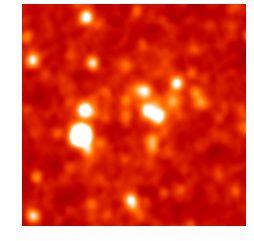
\includegraphics[width=\linewidth]{example_ir}
                \caption{}
                \label{ir}
            \end{subfigure}
            \begin{subfigure}[b]{0.24\linewidth}
                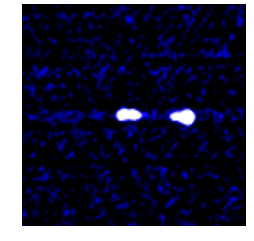
\includegraphics[width=\linewidth]{example_radio}
                \caption{}
                \label{radio}
            \end{subfigure}
            \begin{subfigure}[b]{0.24\linewidth}
                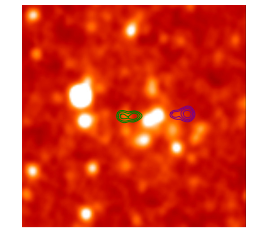
\includegraphics[width=\linewidth]{example_contours}
                \caption{}
                \label{contours}
            \end{subfigure}
            \begin{subfigure}[b]{0.24\linewidth}
                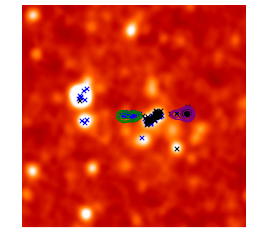
\includegraphics[width=\linewidth]{example_clicks}
                \caption{}
                \label{clicks}
            \end{subfigure}
            \caption{\eqref{ir} Infrared image of subject. \eqref{radio} Radio image of subject. \eqref{contours} Volunteers decide which emissions are from the same source. \eqref{clicks} Volunteers decide where each radio source is located.}
        \end{figure}

        These are stored in a MongoDB database. The raw locations provided by volunteers don't necessarily agree and need to be processed to find a single location for each radio source; Banfield et al.\cite{banfield15} provide code to do this, but their code doesn't find the uncertainty associated with the resulting location and we may want to make use of this uncertainty while learning. It may also not be possible to simply choose the most agreed upon location for a given radio source --- for example, 49\% of the volunteers may believe that location 1 is where the radio source is located, and 51\% may believe that the location is actually location 2. It could be misleading to say that location 2 is the ``true'' location when there is this much disagreement, and so I will have to determine the extent of this problem and subsequently find solutions.

    \subsection*{Forming a classification task}

        The cross-identification problem can be cast as a binary classification problem. The naïve way to do this is to slide a window over the infrared and radio images, where each window has the label $1$ when the window is centred on the radio source and $0$ otherwise. However, this is expensive, especially for larger images. A potentially better way is to identify locations that may host the radio source, and then label these as $1$ if they are the true radio host and $0$ otherwise. I will attempt to identify such potential hosts and classify them in this way. I will also need to find useful features of the potential hosts to use as inputs for the classifier --- examples may include the infrared brightness of the potential hosts, the distance from the potential hosts to the centre of the radio emissions, and so on.

    \subsection*{Training a classifier}

        The final part of the problem is to train a classifier and subsequently perform the classification task. It isn't obvious what kind of classifier to use, but preliminary results suggest that a logistic regression-based approach may be suitable. A logistic regression classifier can be trained on the potential host features, and configured to output the probability that each potential host should have a $1$ label. The potential host with the highest probability is then considered to be the host galaxy. It may also be possible to treat the problem as a computer vision object detection problem on the radio image. If so, then a region-based convolutional neural network may be used to detect the host galaxy. These approaches could even be combined.

    % \textbf{Research question:} Can we use the results of Radio Galaxy Zoo (RGZ), a crowdsourced citizen science project, as training data to learn to automatically identify black hole emissions with their host galaxies?

    % \textbf{Background and related work:} Banfield et al. 2015 and other papers cited in this paper. There's also probably some papers on black hole classification? I should find some of that.

    % \textbf{Technical details:} RGZ data are subjects and classifications in a MongoDB database. I need to convert these into training data, and then use machine learning techniques to complete the task. Preliminary results suggest that techniques building on logistic regression will be the most useful. In second semester, I will investigate active learning on this dataset in the context of the RGZ project.

    \subsection*{Future work}

        This proposal describes the first semester of my honours project. The second semester will focus on some facet of crowdsourced active learning with the Radio Galaxy Zoo, though the specific details of this have not yet been determined and may depend on the results of the first semester. As a result of this, I will need to be thinking about the active learning problem while working on the first semester of the project, and this is reflected in my project plan.

    \subsection*{Project plan}

        \begin{itemize}
            \item February: \begin{itemize}
                    \item Familiarise myself with the dataset.
                    \item Cast the problem as a binary classification problem.
                    \item Understand Kyle Willett's RGZ code accompanying the Banfield et al. 2015 paper.
                \end{itemize}
            \item March: \begin{itemize}
                    \item Convert raw RGZ data into training sets.
                    \item Run RGZ training sets through simple classifiers.
                    \item Read papers on crowdsourced active learning (e.g. Yan et al. 2011\cite{yan11} and Mozafari et al. 2012\cite{mozafari12}).
                    \item Read papers on other astronomical classification problems (e.g. Richards et al. 2012\cite{richards12}).
                    \item Determine the extent of the label disagreement problem. Can we just use majority vote?
                \end{itemize}
            \item April: \begin{itemize}
                    \item Begin writing up problem observations.
                    \item Investigate using metadata and RGZ image structure as features.
                    \item Implement a CNN and understand CNN features with help from computer vision researchers.
                    \item Experiment with different classifiers to find the best classifier to use for the classification task.
                    \item Summarise the crowdsourced active learning papers.
                    \item List weaknesses of crowdsourced active learning papers.
                \end{itemize}
            \item May: \begin{itemize}
                    \item Make a software package for the RGZ classification problem.
                    \item Implement the active learning algorithm from Yan et al. 2011.
                    \item Decide on future work for semester 2.
                    \item Work on making software package user-friendly for astrophysicists.
                    \item Present results (final report and presentation).
                \end{itemize}
        \end{itemize}

\bibliographystyle{plain}
\bibliography{papers}

\end{document}
